\label{ST2}
The Lennard-Jones is an extremely useful potential for computational studies because the Lennard-Jones potential is highly stable and well studied.  Results of new methods are easy to confirm with the Lennard-Jones potential since the properties of the potential are very well known at this point.  Further, the potential is simple to implement and simulate.  A Lennard-Jones system was a first system for using metadynamics to studying nucleation and crystal growth, as Lennard-Jones is known to crystallize to the FCC phase and shows no polymorphs.  However, we wish to extend our use of metadynamics to study nucleation to a system that has more real-world application than Lennard-Jones.  One system we hope to study is water.  Water nucleation and crystallization can be difficult to study as it shows several polymorphs in the crystal phase.  Also, over dozens of water models have been developed for use in MD codes because water is difficult to reproduce with a simple model.  With that said, water is a crucial system to understand and using metadynamics could elucidate why water preferentially freezes to one polymorph over another at different phase points.  To study water, we use the ST2 water model.

\section{Theory and Model}
The ST2 water model, developed by Stillinger et. al. \cite{Stillinger1974}, while controversial, has been widely used to study water with computer simulations.  The model has received a great deal of attention because the model is known to produce a liquid-liquid phase transition near a second critical point in the supercooled state, changing from a high density liquid to a low density liquid.  The ST2 model is a 5-site water model, as shown in Figure \ref{ST2_model}, which means a non-bonded electron pair of the oxygen atom is represented by a virtual site, $L$.  A virtual site is considered an atom of zero mass in simulations, allowing it to add a coulomb interaction to the force field.  
\begin{figure}
	\centering
	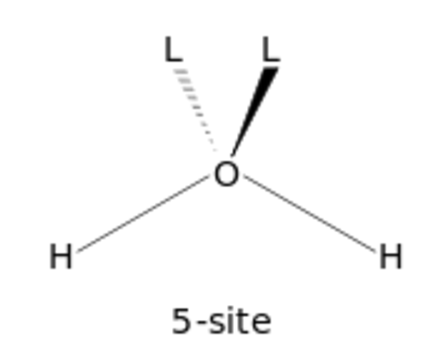
\includegraphics[width=.2\textwidth]{./Figures/Appendix/ST2_diagram.png}
	\hspace{.1\textwidth}
	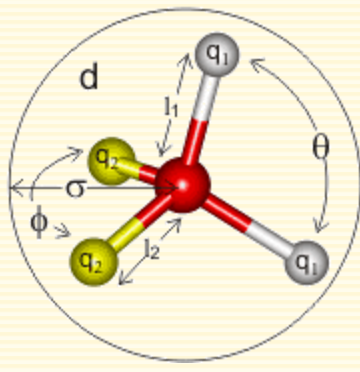
\includegraphics[width=.2\textwidth]{./Figures/Appendix/ST2_model.png}
	\caption[These two figures show a schematic drawing of a 5-site water model.  In the figure, a L site or $q_2$ is a virtual site that represents the non-bonded electron pairs of oxygen.  As a result, the oxygen atom is typically considered with a zero charge and only contains a Lennard-Jones interaction.  Various models use this 5-site model, and fit the parameters such as charge value, bond angles, and bond lengths to fit the model to experimental results.  One such 5-site model is the ST2 model created by Stillinger et. al.]{These two figures show a schematic drawing of a 5-site water model.  In the figure, a L site or $q_2$ is a virtual site that represents the non-bonded electron pairs of oxygen.  As a result, the oxygen atom is typically considered with a zero charge and only contains a Lennard-Jones interaction.  Various models use this 5-site model, and fit the parameters such as charge value, bond angles, and bond lengths to fit the model to experimental results.  One such 5-site model is the ST2 model created by Stillinger et. al. \cite{Stillinger1974}.}
	\label{ST2_model}
\end{figure}
The ST2 water model is unique in that, while most 5-site models' potential is a simple combination of a Lennard-Jones term and a coulomb term, the model introduces a ``switching function,'' $S(r_{12})$, to the coulomb term.  The ``switching function'' alters the strength of the coulomb term depending on distance of the water models, it represents a screening effect.  Thus, the model takes the form of
\begin{equation}
V(1,2) = V_{LJ}(r_{12})+S(r_{12})V_{el}(1,2)
\end{equation}
Where $V(1,2)$ is the potential on water molecule 1 by water molecule 2, $V_{LJ}$ is the Lennard-Jones 6-12 potential caused by the oxygen atoms, $r_{12}$ is the distance between the two molecules oxygen atoms, $S(r_{12})$ is the ST2 switching function (equals 1 for water models like SPC, TIP3P, etc.), and $V_{el}$ is the electronic potential contributed by the coulomb charges on the hydrogens and the virtual sites.
\begin{equation}
V_{LJ}(r_{12}) = 4\epsilon\left[\left(\frac{\sigma}{r_{12}}\right)^{12} - \left(\frac{\sigma}{r_{12}}\right)^6\right]
\end{equation}
where $\sigma$ and $\epsilon$ are fitting parameters for the Lennard-Jones potential.
\begin{equation}
	V_{el}(1,2) = \sum_{\alpha,\beta}^4\frac{q_\alpha q_\beta}{d_{\alpha\beta}(1,2)}
\end{equation}
where $\alpha$ and $\beta$ are indices indicating the four charge sites in the ST2 model. Lastly,
\begin{equation}
S(r_{12}) = \left\{ 
\begin{array}{l l}
0 & \quad r_{12} \le R_L\\
\frac{\left(r_{12}-R_L\right)^2\left(3R_U-R_L-2r_{12}\right)}{\left(R_U-R_L\right)^3} & R_l \le r_{12} \le R_U\\
1 & \quad R_U \le r_{12}
\end{array} \right.
\end{equation}
where $R_L$ is the lower switching limit and $R_U$ is the upper switching limit.  The parameters for this model are as shown in Table $\ref{ST2_parameters}$.
\begin{table}
	\centering
	\caption[Table summarizing the parameters used for the ST2 model created by Stillinger et. al.]{Table summarizing the parameters used for the ST2 model created by Stillinger et. al. \cite{Stillinger1974}.}
	\label{ST2_parameters}
	\begin{tabular}{ c c c c }
		Parameter& ST2 Value & Parameter & ST2 Value \\
		\hline	
		\hline		
		\\
		$r_{OH} $(\AA)      & 1.0    & $\epsilon (kJ/mol)$ & .31694 \\
		$\theta_{HOH} (^o)$ & 109.47 & $q_L$ (C)           & -.24357 \\
		$r_{OL} $(\AA)      & 0.8    & $q_H$ (C)           & .24357 \\
		$\theta_{LOL} (^o)$ & 109.47 & $R_L$ (\AA)         & 2.0160 \\
		$\sigma$ (\AA)      & 3.1    & $R_U$ (\AA)         & 3.1287\\
		\hline 
	\end{tabular}
\end{table}

This model has not previously been implemented into GROMACS.  The current distribution of GROMACS does not even have 5-site water molecules included, instead models such as TIP5P (a 5-site model) was considered as 5 individual bonded atoms rather than as a water model.  Thus, we added both the TIP5P model as a water model and by extension added the ST2 water model to GROMACS list of water models in the OPSLAA topology class.  The model is added such that coulomb interactions can be handled as both cut-off coulomb forces or handled with Ewald summations.  No acceleration methods have been implemented with ST2 water as with the other models, but the model is fully compatible with OpenMP and MPI parallelization.  The model was benchmarked at 300 K, with ambient pressure, and compared to the original work of Stillinger et. al. \cite{Stillinger1974}.  Both the structural and dynamical properties were confirmed.  We then combined the ST2 model built into GROMACS with the metadynamics build of GROMACS in order to study ST2 water with metadynamics.

\section{Preliminary Results}
At this point, we have tested our ST2 water model with our metadynamics implementation.  The system was composed of 262 water molecules, or 1310 atoms.  An NPT simulation was used to equilibrate the system to a box with 1.95 nm edge, or a density of 1050 kg/$m^3$.  The system was then equilibrated with a 1 ns NVT simulation at 300 K.  The metadynamics simulation used a step tolerance of 10$^8$, initial step, $\delta$ of .0001, maximum steps per penalty of 7000, penalty height of 5 kJ/mol, penalty width squared of .1 nm$^2$, and maximum penalties of 20,000.  The simulation results are displayed in Figure \ref{st2}.
\begin{figure}
	\centering
	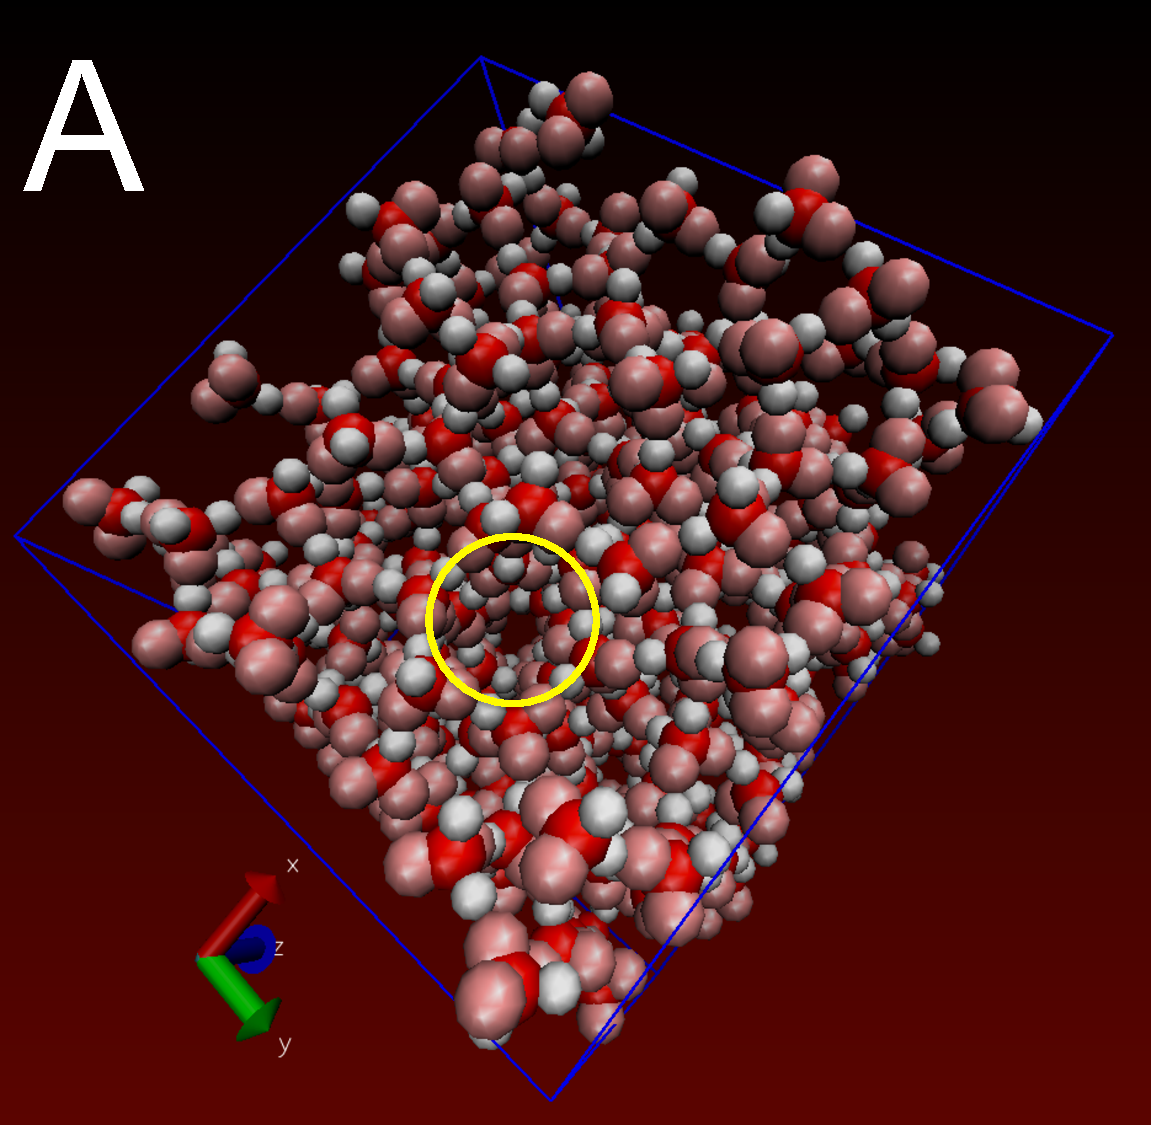
\includegraphics[width = .45\textwidth]{./Figures/Appendix/st2_water_final.pdf}
	\hspace{.03\textwidth}
	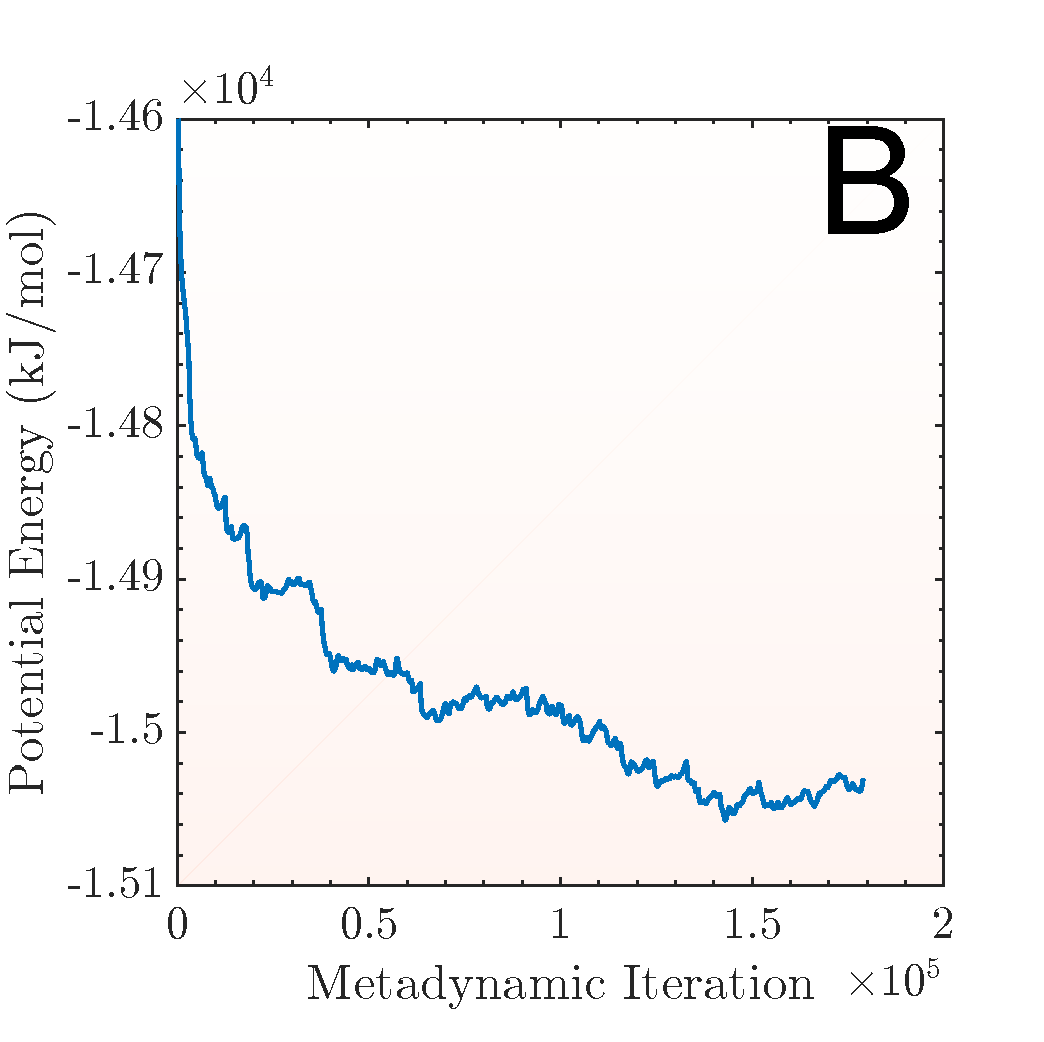
\includegraphics[width = .45\textwidth]{./Figures/Appendix/st2_landscape.pdf}
	\caption{These two figures show the preliminary results for using the metadynamics method with a system of water dictated by the ST2 water model.  Figure A shows the final configuration of the system after the simulation.  The red atoms are oxygen atoms, the white atoms are hydrogen atoms, and the pink atoms are the virtual charges on the oxygen atoms (which GROMACS treats similar to atoms).  The yellow circle is to emphasis a lack of atoms through the simulation box, which seems indicative of structure water molecules in this region. Figure B shows the potential energy of the system during the simulation.}
	\label{st2}
\end{figure}

Figure \ref{st2} A shows a visualization of the final configuration of the system after metadynamics have been performed.  From visual inspection, we found that the simulation begins amorphous (liquid state), as expected, and then after the simulation some amount of order is found in the system.  The yellow circle is to emphasis a region we believe to contain order.  The region appears to have hexagonal ordering typical of ice.  However, unlike the Lennard-Jones simulations, ordering is not visually obvious, especially since ice has several polymorphs.  There is likely multiple ice phases in this system which makes identification of order difficult.  More than likely in order to understand this simulation we will need to use both the sixth and fourth order bond orientational order parameter, $\bar{q}_6$ and $\bar{q}_4$.  

Figure \ref{st2} B shows the potential energy of the system during the simulation.  The landscape is clearly more complicated than the landscape sampled for the Lennard-Jones system.  This is to be expected as ST2 is the more complicated system.  At this point, we feel a significantly longer trajectory will be necessary before further analysis can be performed.  However, from our understanding by comparing the monoatomic Lennard-Jones to the binary Lennard-Jones landscapes in Chapter \ref{compare landscapes}, we can conclude that the system is most likely crystallizing since the landscape is more comparable to the crystal forming monoatomic Lennard-Jones.